% -*- coding: utf-8 -*-
%

% reset all acronym expansions
\acresetall

%%%%%%%%%%%%%%%%%%%%%%%%%%%%%%%%%%%%%%%%%%%%%%
\chapter{Implementation}
\label{ch:Implementation}
%%%%%%%%%%%%%%%%%%%%%%%%%%%%%%%%%%%%%%%%%%%%%%

When building a platform for \ac{ppml}, we must go beyond the traditional steps in data processing mentioned in Section \ref{sec:PrivacyImplicationsPersonalDataProcessing} and in Figure \ref{fig:crisp-dm}, and also have an increased care when preprocessing data to incorporate the cryptographic techniques.

This Chapter describes the work that was done in implementing a \ac{ppml} platform. In Section \ref{sec:StructureImplementation}, we start off with a description of the structure we followed in implementing and evaluating the platform.
In Section \ref{sec:DatasetsImplementation}, we offer a description of the datasets chosen to test our platform. Then, we explain the preprocessing that was done to those datasets, in Section \ref{sec:DataPreProcessingImplementation}.
Section \ref{sec:BaselineImplementation} presents the baseline implementation of the chosen \ac{ml} algorithms, resorting to a widely used \ac{ml} toolkit for Python.
In Section \ref{sec:CryptoDomainImplementation}, we present the cryptographic protocols used, why we used them, and how we implemented them, mentioning which toolkits were used.
For understanding the applicability of the solution developed, we detail in Section \ref{sec:usecaseHealthcare} a use case for our implementation. Finally in Section \ref{sec:components} we present a possible usage for our implementation, in the form of a toolkit that could be used in a business environment.


  %%%%%%%%%%%%%%%%%%%%%%%%%%%%%%%%%%%%%%%%%%%%%%%%%%%%%%%%%%%%%%%%%%%%%%%%%%%%%
  %
%%%%%                        THE BEGINNING
 %%%
  %


\input content/4040-api.tex
\input content/3020-use_case.tex



%%%%%%%%%%%%%%%%%%%%%%%%%%%%%%%%%%%%%%%%%%%%%%%%%%%
\section{Structure}
\label{sec:StructureImplementation}
%%%%%%%%%%%%%%%%%%%%%%%%%%%%%%%%%%%%%%%%%%%%%%%%%%%

The process of implementing and testing a \ac{ppml} platform can be achieved in a number of steps. The plan we designed was composed of three steps, each with three processes that are repeated for all steps.

\begin{itemize}

	\item \textbf{Step 1}: Use a toolkit (\textit{scikit-learn}) to implement baseline versions of the chosen \ac{ml} algorithms. Each of the processes were performed in black boxes\footnote{A black box is a device, system or object which can be viewed in terms of its inputs and outputs, without any knowledge of its internal workings.} supplied by the toolkit:
	\begin{enumerate}
		\item Compute the model using the training set.
		\item Use the model to predict the labels of the testing set.
		\item Evaluate the performance of the model by comparing predicted labels with the real ones.
	\end{enumerate}
	\item \textbf{Step 2}: Write scripts implementing the \ac{ml} algorithms that explicitly contain all the equations for the processes described above.
	\item \textbf{Step 3}: Rewrite the scripts from Step 2 using cryptographic techniques to perform the necessary computations, that add protections for all the processes described above.
\end{itemize}

It is important to mention that the processes in Steps 2 and 3 where implemented in reverse order, not only because training is more complex that prediction, which in turn is more complex that evaluation, but also because this new ordering better matches the purpose and logic of implementing them using cryptographic techniques for privacy-preserving purposes. Figure \ref{fig:steps} presents a visual representation of the structure we followed, and show what was left for future work.

\begin{figure}[ht]
    \centering
    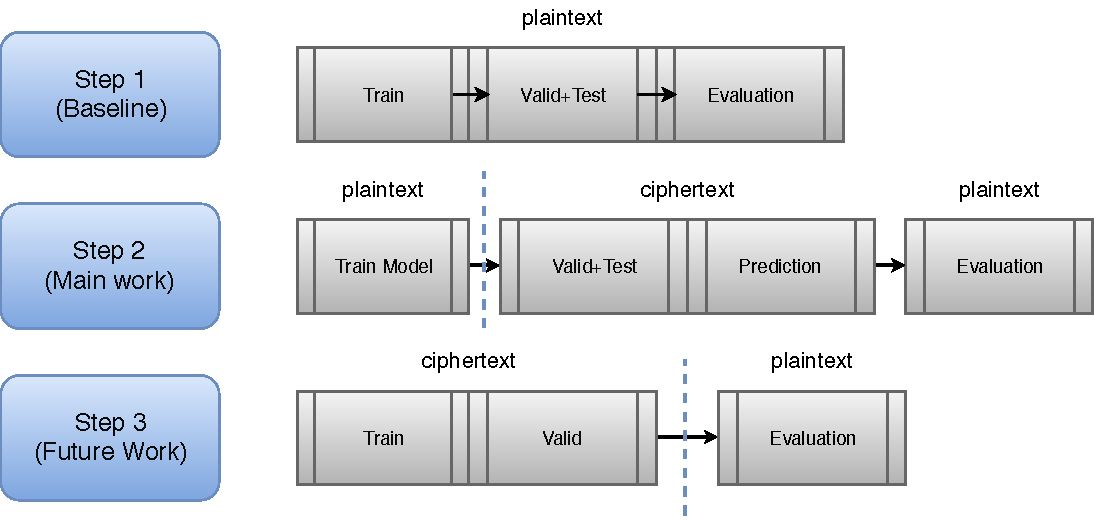
\includegraphics[width=0.80\textwidth]{images/ImplementationSteps.pdf}
    \caption{Steps and Processes of the implementation.}
    \label{fig:steps}
 \end{figure}


%%%%%%%%%%%%%%%%%%%%%%%%%%%%%%%%%%%%%%%%%%%%%%%%%%%

\input content/3010-implementation.tex



  %%%%%%%%%%%%%%%%%%%%%%%%%%%%%%%%%%%%%%%%%%%%%%%%%%%%%%%%%%%%%%%%%%%%%%%%%%%%%
  %
%%%%%                        LAST SECTION
 %%%
  %

  
%%%%%%%%%%%%%%%%%%%%%%%%%%%%%%%%%%%%%%%%%%%%%%
\section{Summary}
\label{sec:SummaryImplementation}
%%%%%%%%%%%%%%%%%%%%%%%%%%%%%%%%%%%%%%%%%%%%%%


In this Chapter, we discussed the implementation of a privacy-preserving \ac{ml} platform. We started by describing the datasets chosen to evaluate the platform in Section \ref{sec:DatasetsImplementation}, and then we explained the preprocessing step in Section \ref{sec:DataPreProcessingImplementation}.
Section \ref{sec:BaselineImplementation} presented the implementation of the baseline for the chosen \ac{ml} algorithms.
In Section \ref{sec:CryptoDomainImplementation}, we detailed which cryptographic protocols we used, why we used them, and how we implemented them, mentioning which toolkits were used.
For understanding the uses of the solution developed, we detailed in Section \ref{sec:usecaseHealthcare} a use case for our implementation, and finally in Section \ref{sec:components} we presented a possible usage for our implementation, in the form of a toolkit that could be used in a business environment.


  %
 %%%
%%%%%                        THE END
  %
  %%%%%%%%%%%%%%%%%%%%%%%%%%%%%%%%%%%%%%%%%%%%%%%%%%%%%%%%%%%%%%%%%%%%%%%%%%%%%
